\documentclass{article}
\usepackage[margin=1in]{geometry}
\usepackage{graphicx}
\usepackage{xcolor}
\usepackage{float}
\graphicspath{{..} {./images}}

\renewcommand{\contentsname}{\vspace*{-2\baselineskip}}

\begin{document}
\begin{titlepage}
	\centering
	{\huge Lab 1 - Introduction to Software-Defined Radio}\\[0.25 in]
	
\includegraphics[width=0.6\textwidth]{ua_logo.png}\\[0.25 in]
	{\large \textbf{ECE 531 - Software Defined Radio\\[0.25 in]
	Spring 2025\\[0.25 in]}}
	{\large Owen Sowatzke, osowatzke@arizona.edu\\[0.05 in]
	Department of Electrical \& Computer Engineering\\[0.05 in]
	University of Arizona, Tucson, AZ 85721\\[0.5 in]}
	\textcolor{blue}{
	\noindent\hrulefill
	\tableofcontents
	\noindent\hrulefill
	}
\end{titlepage}

\section{Introduction}
Introduction to the laboratory experiment, including a brief description of the objectives and goals.

SDR flowgraphs 

GNU Radio simulation

Topics:

\begin{itemize}
	\item sampling rates
	\item complex samples
	\item interpolation
	\item decimation
	\item noise analysis
\end{itemize}

\section{Procedure}
% Detailed explanation of the laboratory experiment, including the design, implementation, and testing of the system.

In this lab, we investigate the effects of sampling rates on a sinusoid signal. We, then, investigate how complex sampling differs from real sampling. Next, we observe the spectrum of the sinusoid, while varying its frequency. Then, we examine the effects of I/Q imbalance on a complex-sampled signal.

\subsection{Sampling Rates \label{subsection::sampling_rates}}

In this experiment, we examine the effects of sampling rate. To perform this experiment, we construct the GNU radio companion (GRC) flowchart shown in Figure \ref{fig::sampling_rates_experiment}. We, then, use the "Time" and "Frequency" tabs of the QT GUI to examine the sampled signal.

\begin{figure}[H]
	\centerline{\fbox{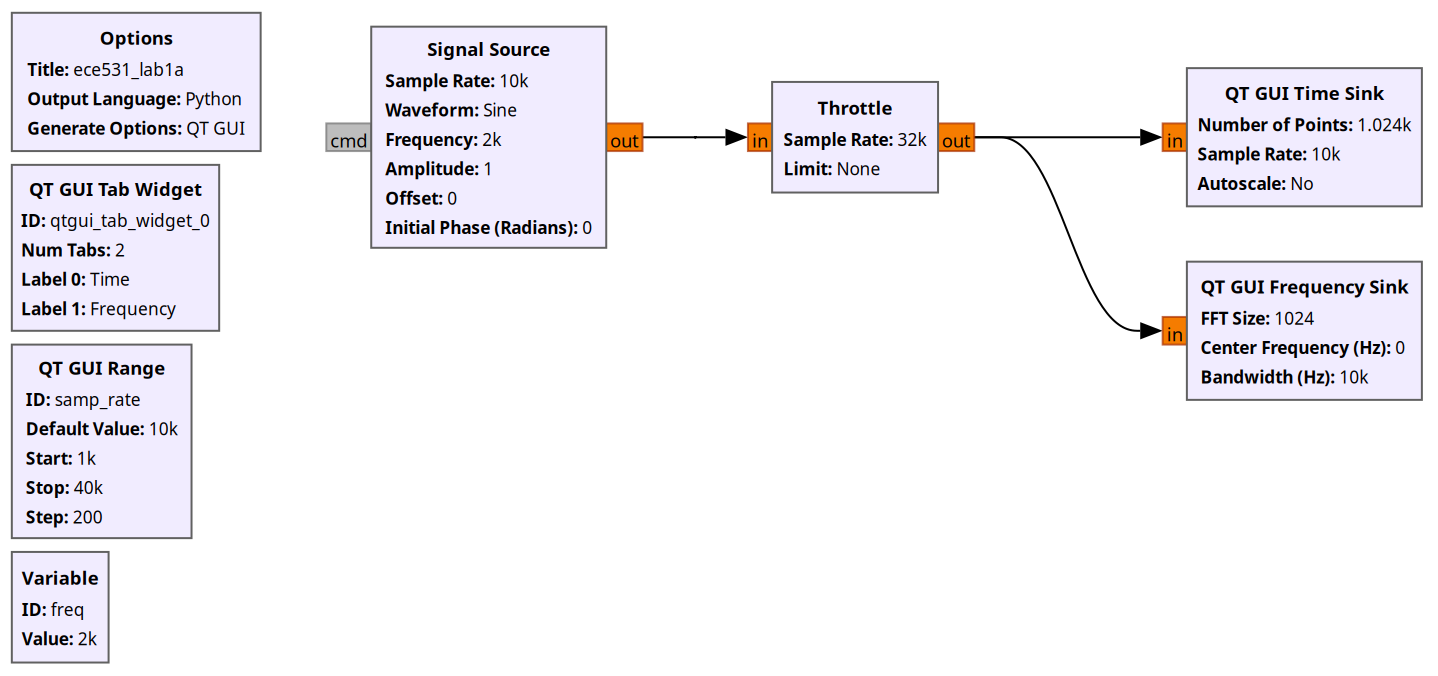
\includegraphics[width=0.7\textwidth]{sampling_rates_experiment.png}}}
	\caption{Setup for Sampling Rate Experiment}
	\label{fig::sampling_rates_experiment}
\end{figure}

We start by examining the signal when it is sampled at the 10 kHz default sample rate. We qualitatively analyze the time-domain signal by comparing it to an ideal sinusoid. We, then, measure the frequency of the signal. Next, we increase the sample rate to 40 kHz and compare the updated time and frequency plots to the previously collected data. Finally, we decrease the sample rate to 3.5 kHz and examine the frequency of the sampled signal.

\subsection{Complex Sampling \label{subsection::complex_sampling}}

In this section, we examine how complex sampling differs from real sampling. To perform our analysis, we modify the data types of the blocks in the GRC flowchart shown in Figure \ref{fig::sampling_rates_experiment}. The updated blocks use a "Complex Float 32" data type instead of a "Float 32" data type. Figure \ref{fig::complex_sampling_experiment} shows the updated block diagram. Note that the port colors have changed from orange to blue to reflect the change in data type.

\begin{figure}[H]
	\centerline{\fbox{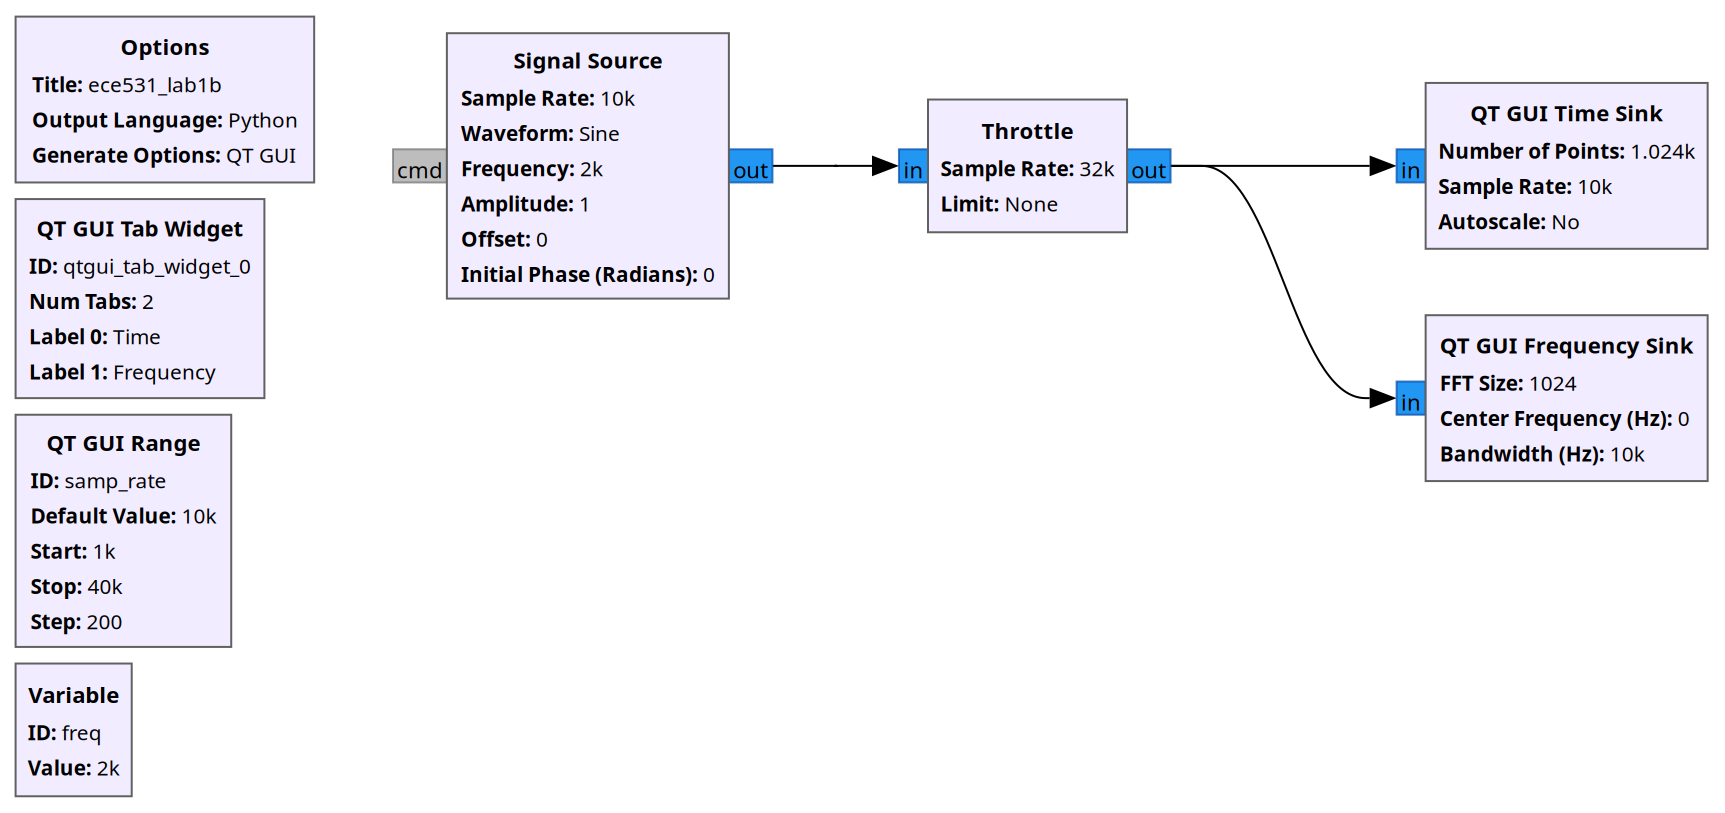
\includegraphics[width=0.7\textwidth]{complex_sampling_experiment.png}}}
	\caption{Setup for Complex Sampling Experiment}
	\label{fig::complex_sampling_experiment}
\end{figure}

Using the updated block diagram, we compare the updated frequency spectrum to the spectrum collected in subsection \ref{subsection::sampling_rates}, noting what happens to the positive and negative frequency components. We, then, investigate the time-domain signals and measure the phase between them. Next, we examine the signal amplitude on each channel while varying the sampling frequency from 10kHz to 40kHz. At the 40kHz sampling rate, we measure the frequency peak. Then, we measure the frequency peak at a 4kHz sampling rate. Finally, we continue decreasing the sampling rate and explain the location of the frequency peak.

\subsection{Frequency Observations}

In contrast to the previous sections, we now vary the frequency of the source while keeping the sampling rate constant. The experiment performed here reinforces the results of the previous sections and is performed on both real and complex-sampled data.
 
\subsubsection{Complex-sampled Flowgraph \label{subsection::frequency_observations_complex_sampling}}

The updated GRC flowchart for complex sampling is shown in Figure \ref{fig::frequency_observations_complex_sampling}. Compared with the previous flowchart, the sinusoid frequency can now be controlled with a slider.

\begin{figure}[H]
	\centerline{\fbox{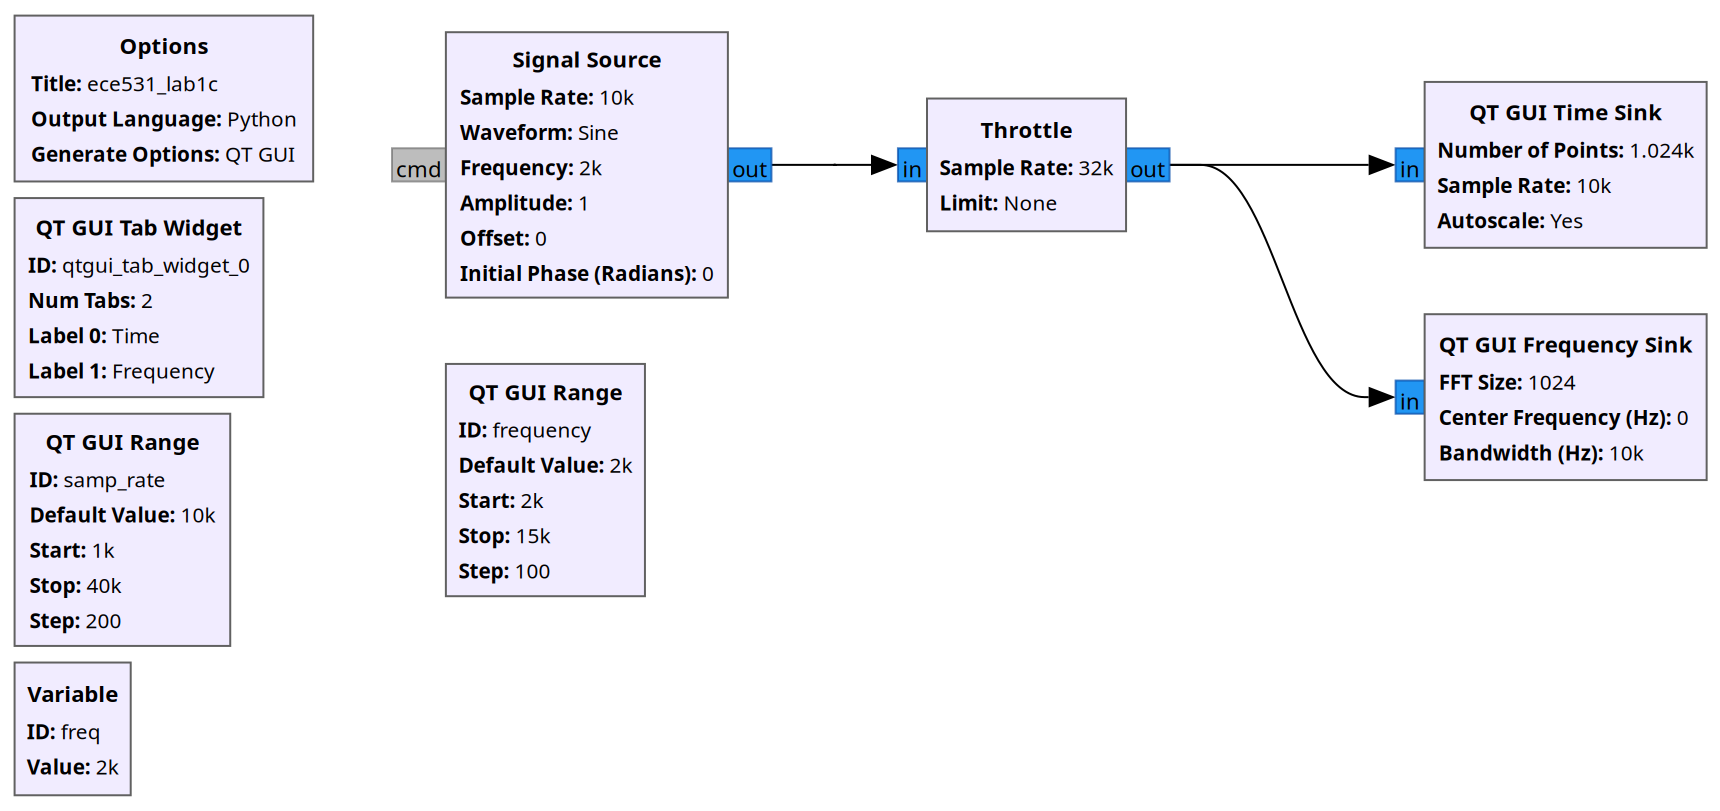
\includegraphics[width=0.7\textwidth]{frequency_observations_complex_sampling.png}}}
	\caption{Complex-sampled Frequency Observations}
	\label{fig::frequency_observations_complex_sampling}
\end{figure}

Using the updated flowchart, we vary the sinusoid frequency over its full range (from 2kHz to 15kHz), while observing the resulting spectrum. Based on the collected data, we notate any anomalies and describe why they occur. 

\subsubsection{Real-sampled Flowgraph}

We also investigate real-sampling using the flowchart shown in Figure \ref{fig::frequency_observations_real_sampling}. The flowchart is identical to the one shown in Figure \ref{fig::frequency_observations_complex_sampling} except for the data types which have been modified from "Complex Float 32" to "Float 32".

\begin{figure}[H]
	\centerline{\fbox{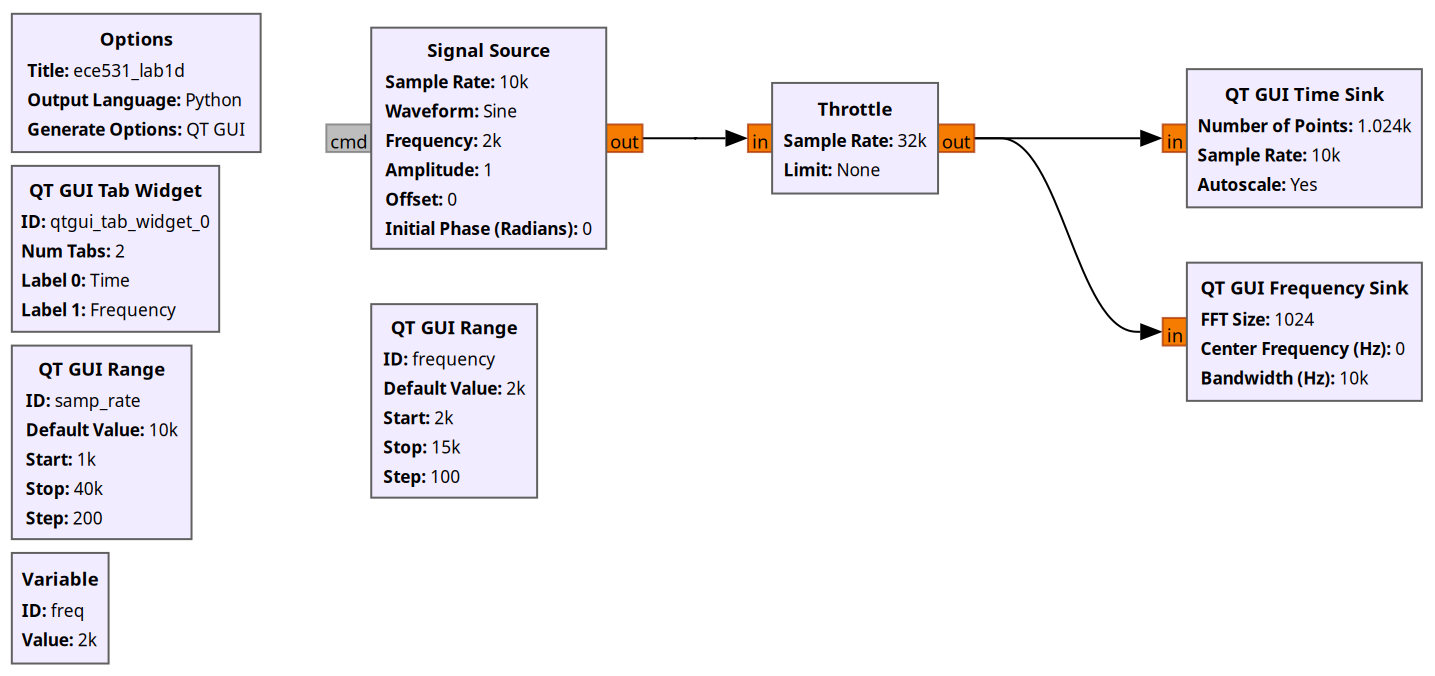
\includegraphics[width=0.7\textwidth]{frequency_observations_real_sampling.png}}}
	\caption{Real-sampled Frequency Observations}
	\label{fig::frequency_observations_real_sampling}
\end{figure}

Using the above flowchart, we vary the frequency of the sinusoid from its default value (10 kHz) to its maximum value (15 kHz). We observe the resulting spectrum and compare to the results we observed in Section \ref{subsection::frequency_observations_complex_sampling}.

\subsection{I/Q Imbalance}

In this section, we investigate the effect of I/Q imbalance on complex sampling. I/Q imbalance refers to a gain-phase mismatches in the I (in-phase) and Q (quadrature) paths. These gain-phase mismatches degrade the sampled signal and result in distortion. Figure \ref{fig::iq_imbalance_experiment} shows the GNU radio flowchart used to investigate I/Q imbalance.

\begin{figure}[H]
	\centerline{\fbox{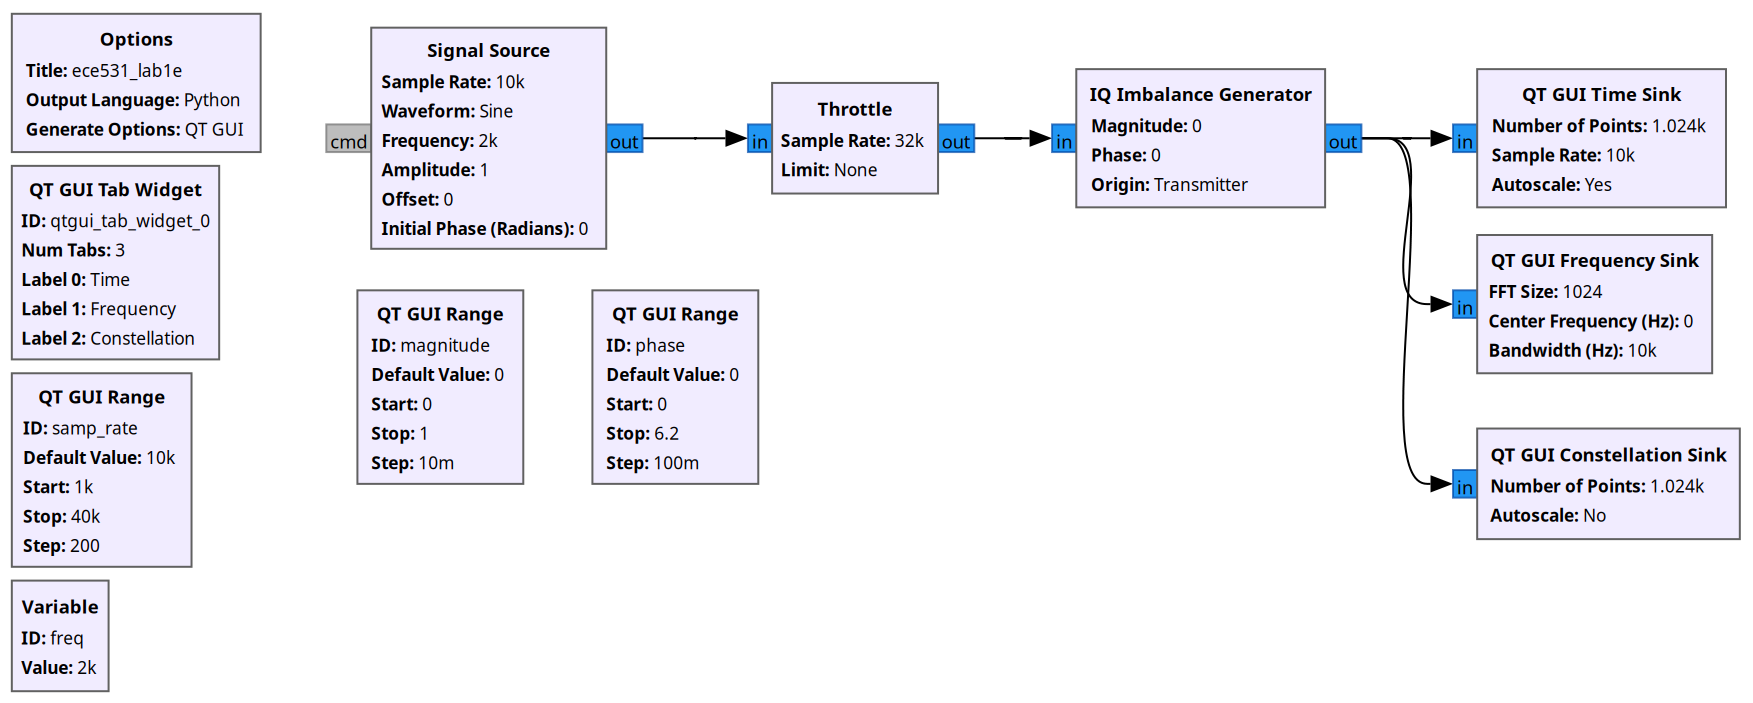
\includegraphics[width=0.7\textwidth]{iq_imbalance_experiment.png}}}
	\caption{I/Q Imbalance Experiment}
	\label{fig::iq_imbalance_experiment}
\end{figure}

With the experiment setup, we first execute with the default values (no gain and phase imbalance) and verify the results are identical to those collected previously. Next, we observe the spectrum while independently varying the gain and phase imbalances - notating what occurs and why. Then, we observe the captured constellation while independently varying the frequency, magnitude, and phase. For each variable that we vary, we log what happens to the received constellation.  

\subsection{Adding Noise}

Building off the flowchart shown in Figure \ref{fig::complex_sampling_experiment}, we add noise to the sinusoidal signal. The resulting flowchart is shown in Figure \ref{fig::noise_experiment}.

\begin{figure}[H]
	\centerline{\fbox{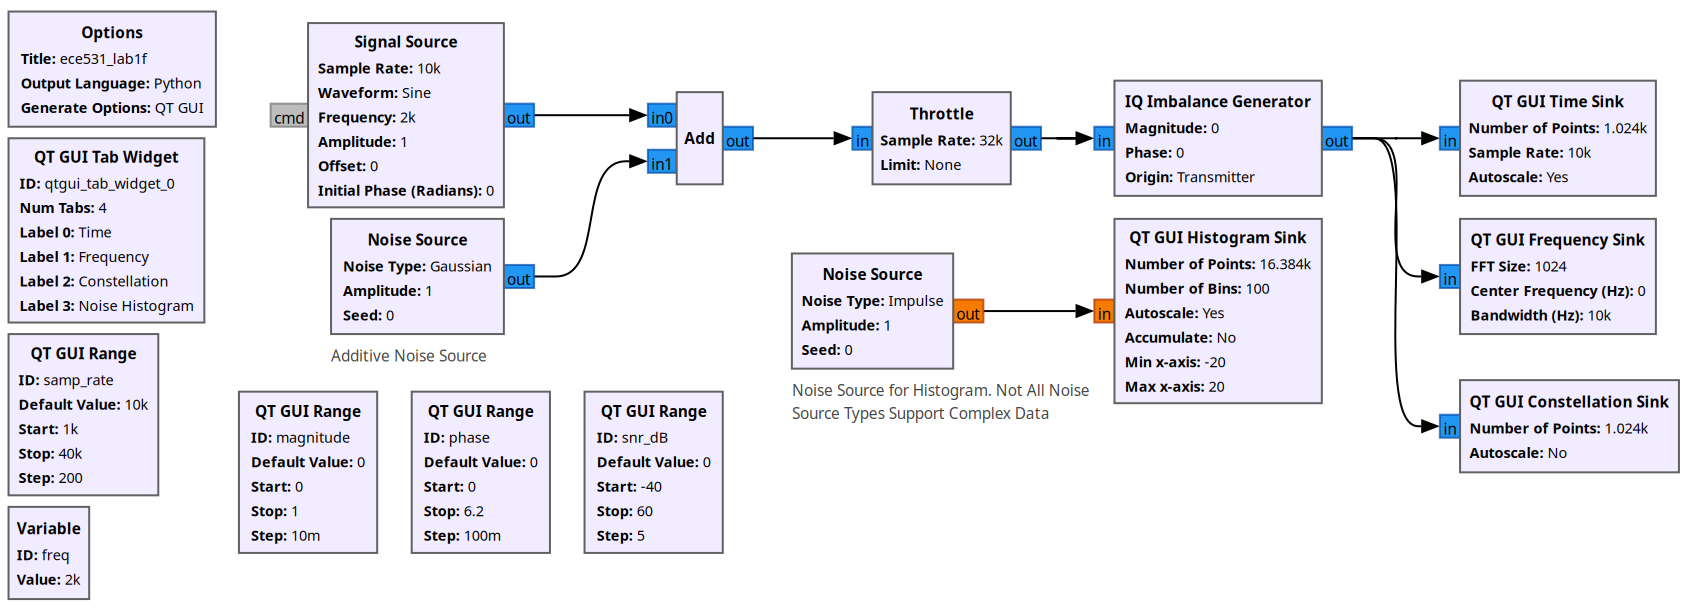
\includegraphics[width=0.7\textwidth]{noise_experiment.png}}}
	\caption{Noise Experiment}
	\label{fig::noise_experiment}
\end{figure}

Using the updated flowchart, we explore the effects of the added noise in the time-domain signal, frequency spectrum, and received constellation points. Next, we use the histogram tab to verify the probability density function (pdf) of each noise source type.

\subsection{Interpolation and Decimation}

For the final experiment, we investigate and decimation, which are used to resample singals. The flowchart used for this analysis is given in Figure \ref{fig::interpolation_and_decimation_experiment}.

\begin{figure}[H]
	\centerline{\fbox{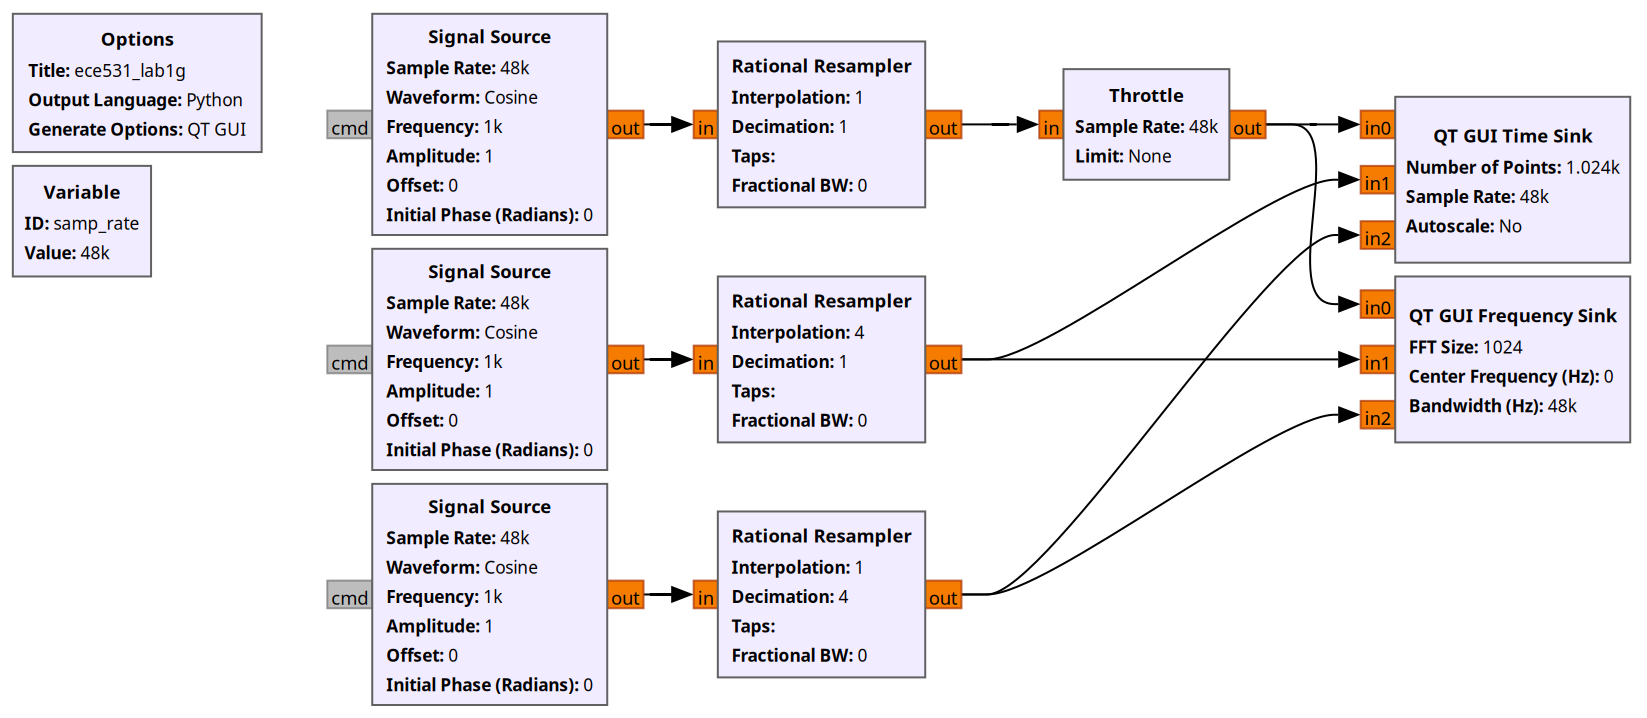
\includegraphics[width=0.7\textwidth]{interpolation_and_decimation_experiment.png}}}
	\caption{Interpolation and Decimation Experiment}
	\label{fig::interpolation_and_decimation_experiment}
\end{figure}

Using the above flowchart, we observe the time and frequency domain outputs and compare the differences between each of the resampled signals. We specifically concentrate on the differences we observe in the frequency spectrum and identify the relationship between each of the signals in the frequency domain.

\section{Results}
% Results and discussion of the laboratory experiment, including captured outputs, observations, and responses to laboratory questions.

\subsection{Sampling Rates}

Using the GNU flowchart shown in Figure \ref{fig::sampling_rates_experiment}, we can view the sampled signal in the time-domain. With a 10 kHz sample rate, the resulting signal is shown in Figure \ref{fig::sampling_rates_time_domain_10k_samp_rate}.

\begin{figure}[H]
	\centerline{\fbox{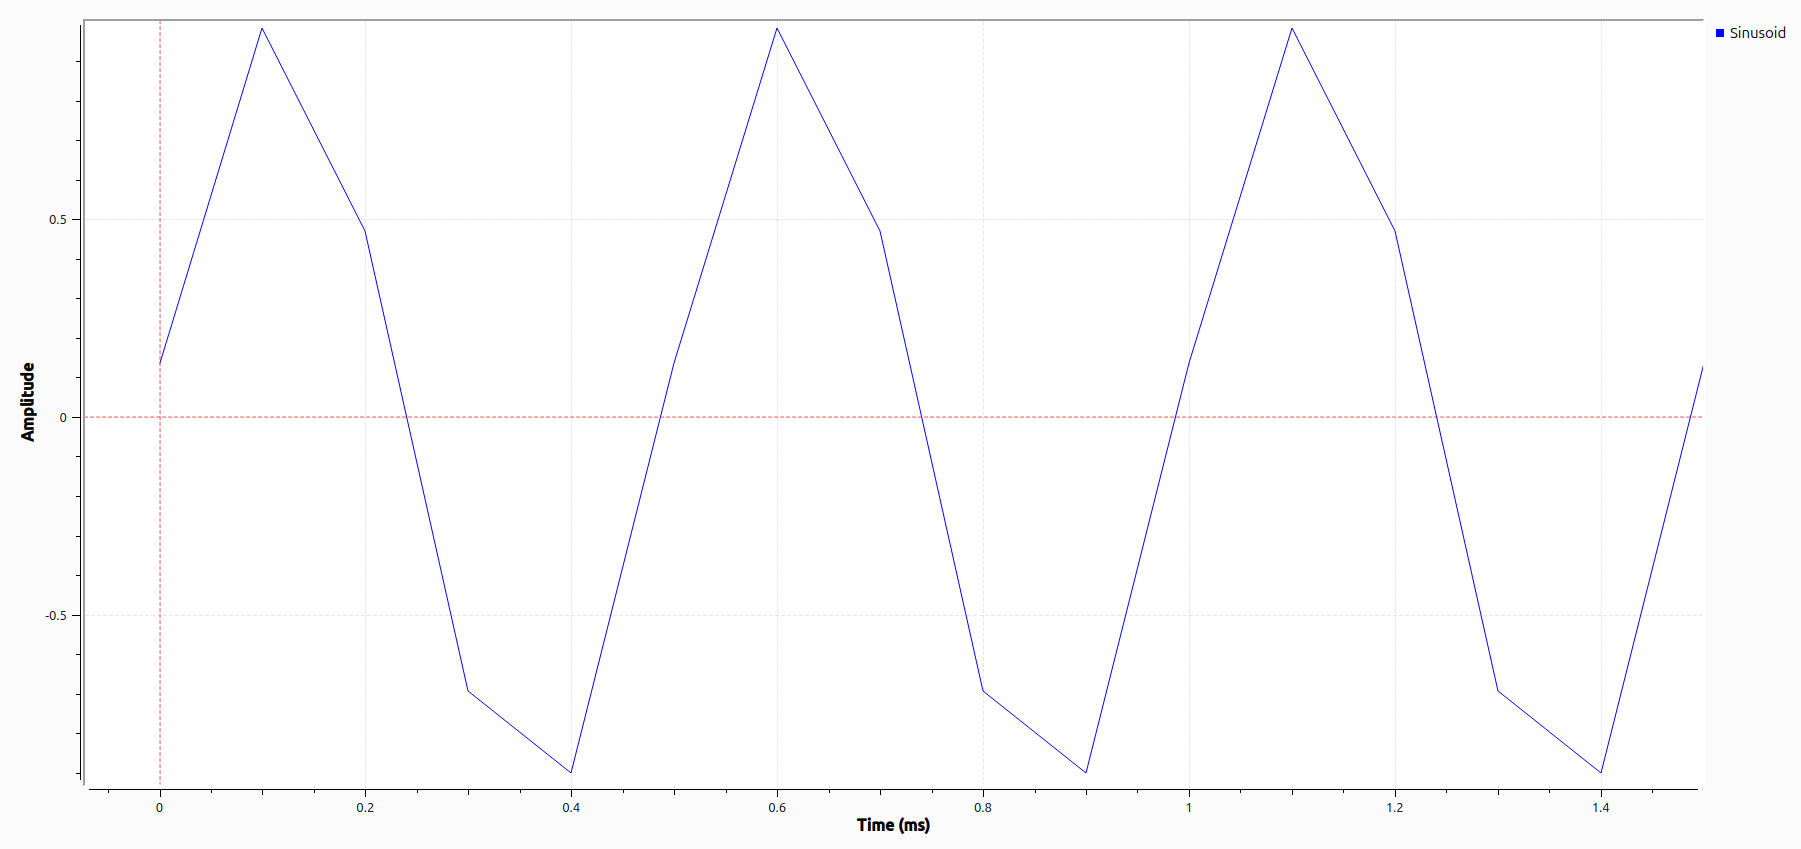
\includegraphics[width=0.7\textwidth]{sampling_rates_time_domain_10k_samp_rate.png}}}
	\caption{Time-Domain Capture of Sinusoid Sampled at 10 kHz}
	\label{fig::sampling_rates_time_domain_10k_samp_rate}
\end{figure}

Reviewing the time domain data, we see that the signal is periodic with a period of 0.5 ms, which is consistent with the 2 kHz sinusoid frequency. We also see the samples are separated by 0.1 ms, which is consistent with the 10 kHz sampling rate. Compared to a continuous time sinusoid, we note that the sine looks jagged due to the linear interpolation between samples. However, we can clearly tell that it is a sinusoid.

Figure \ref{fig::sampling_rates_freq_domain_10k_samp_rate} shows the spectrum of the sampled signal. Examining the frequency response, we see that it peaks at $\pm$ 2 kHz, which is consistent with the sinusoid's frequency.

\begin{figure}[H]
	\centerline{\fbox{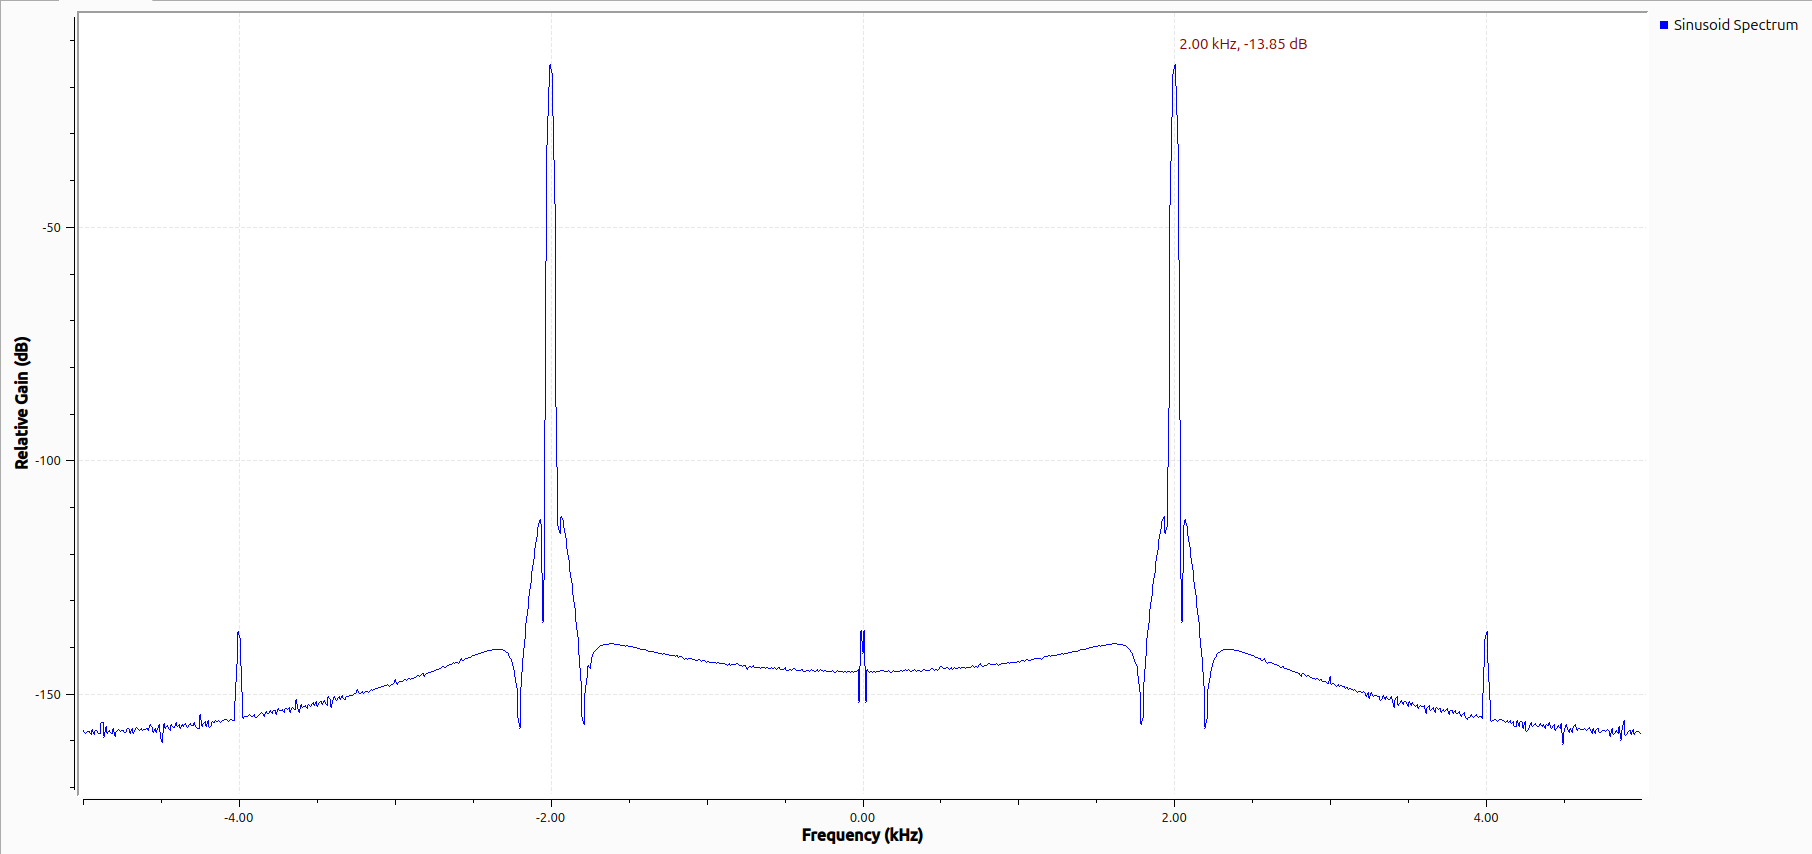
\includegraphics[width=0.7\textwidth]{sampling_rates_freq_domain_10k_samp_rate.png}}}
	\caption{Spectrum of Sinusoid Sampled at 10 kHz}
	\label{fig::sampling_rates_freq_domain_10k_samp_rate}
\end{figure}

Next, we examine the frequency response when the sampling rate is increased to 40 kHz. The updated frequency response is shown in Figure \ref{fig::sampling_rates_freq_domain_40k_samp_rate}. Examining the updated frequency response, we see that it peaks at $\pm$ 2 kHz, which is identical to the frequency it previously peaked at. The biggest difference in the frequency responses is their span. The previously collected data spanned from $\pm$ 5 kHz, while the newly collected data spans from $\pm$ 10 kHz.

\begin{figure}[H]
	\centerline{\fbox{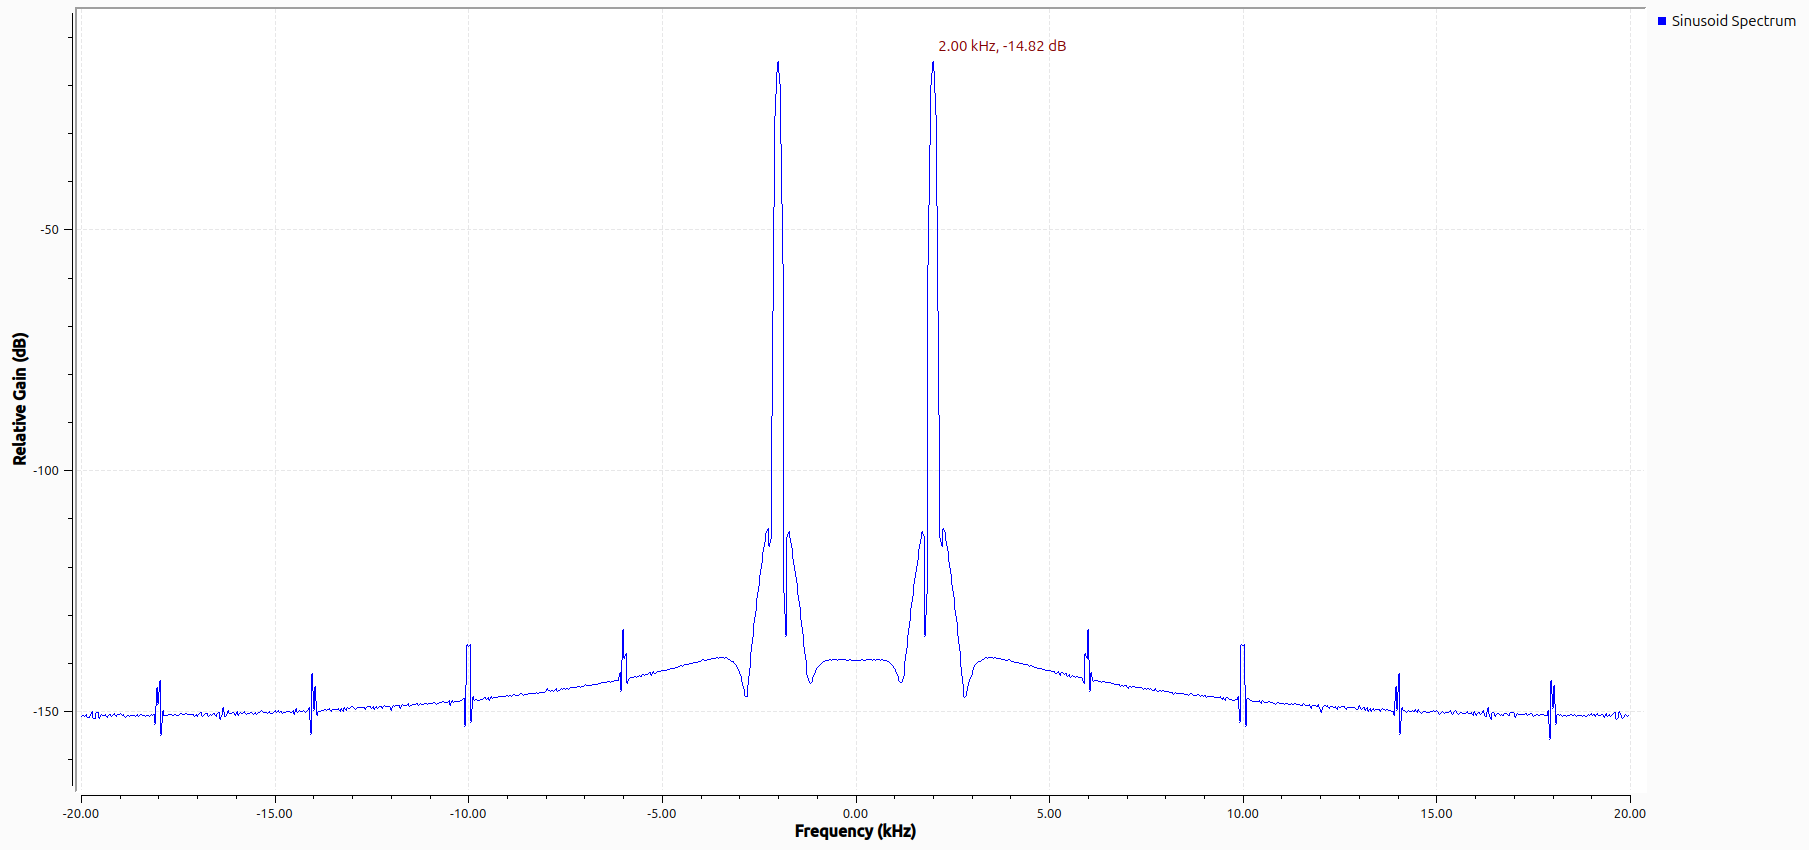
\includegraphics[width=0.7\textwidth]{sampling_rates_freq_domain_40k_samp_rate.png}}}
	\caption{Spectrum of Sinusoid Sampled at 40 kHz}
	\label{fig::sampling_rates_freq_domain_40k_samp_rate}
\end{figure}

After increasing the sample rate to 40 kHz, the scope capture looks much more sinusoid-like. This is because there are more samples per period of the sinusoid, which results in less interpolation between points. The updated scope capture is shown in Figure \ref{fig::sampling_rates_time_domain_40k_samp_rate}.

\begin{figure}[H]
	\centerline{\fbox{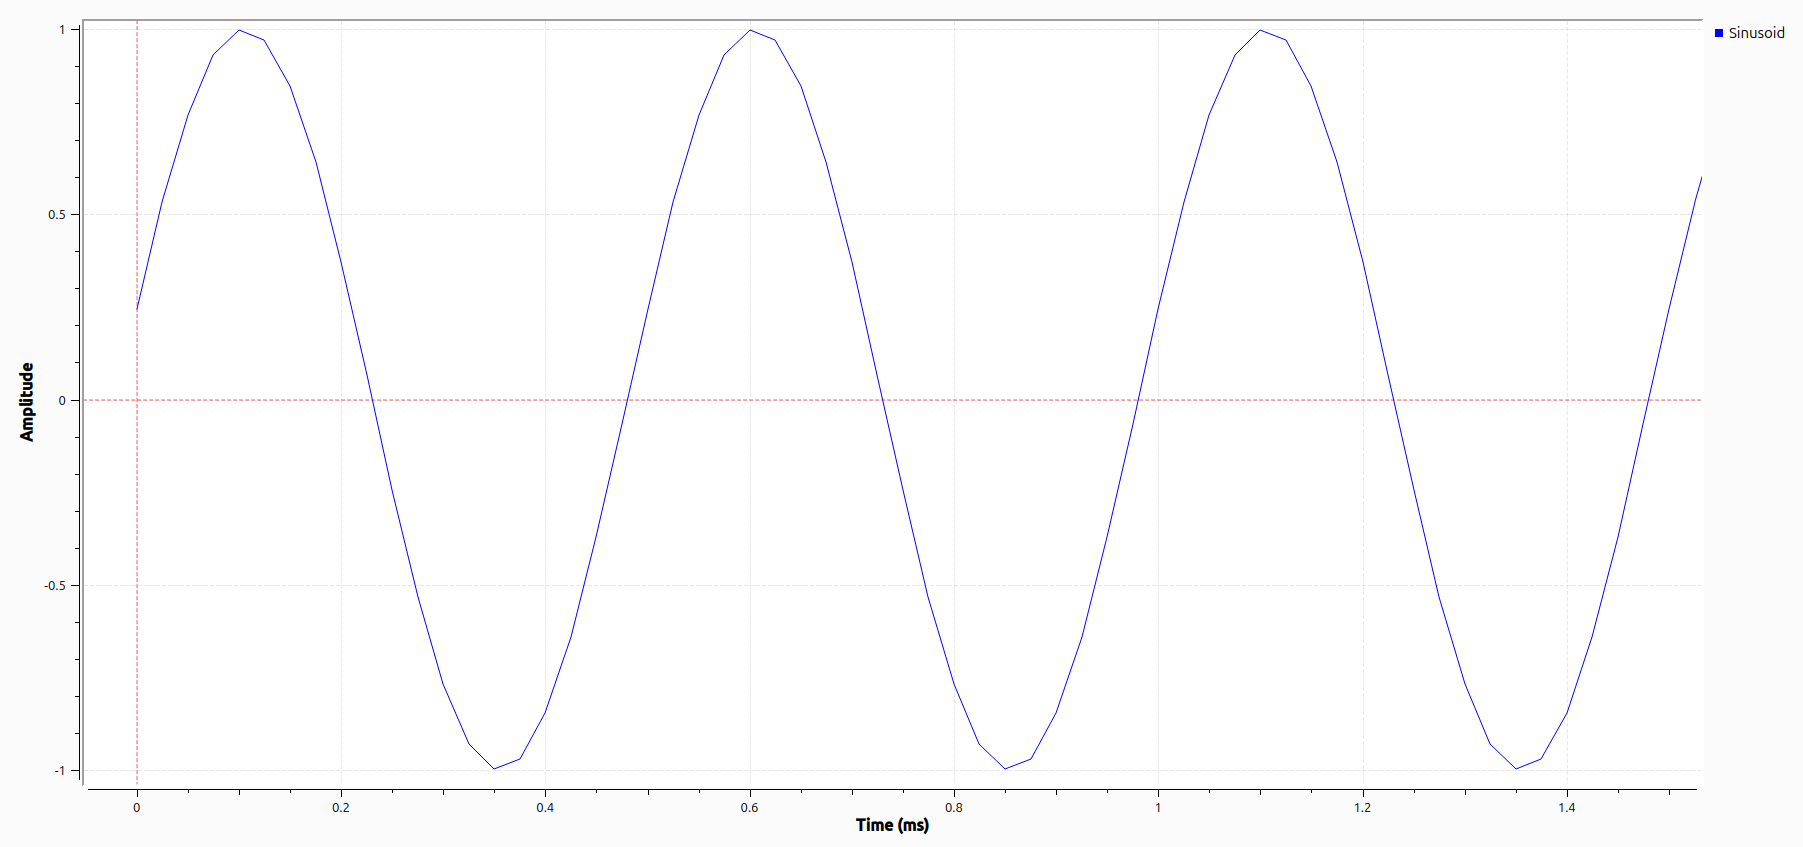
\includegraphics[width=0.7\textwidth]{sampling_rates_time_domain_40k_samp_rate.png}}}
	\caption{Time-Domain Capture of Sinusoid Sampled at 40 kHz}
	\label{fig::sampling_rates_time_domain_40k_samp_rate}
\end{figure}

Now, we adjust the sample rate to 3.5 kHz and measure the peak of the frequency response. We see that the peak is at 1.5 kHz instead of 2 kHz. This is illustrated in Figure \ref{fig::sampling_rates_freq_domain_3_5k_samp_rate}.

\begin{figure}[H]
	\centerline{\fbox{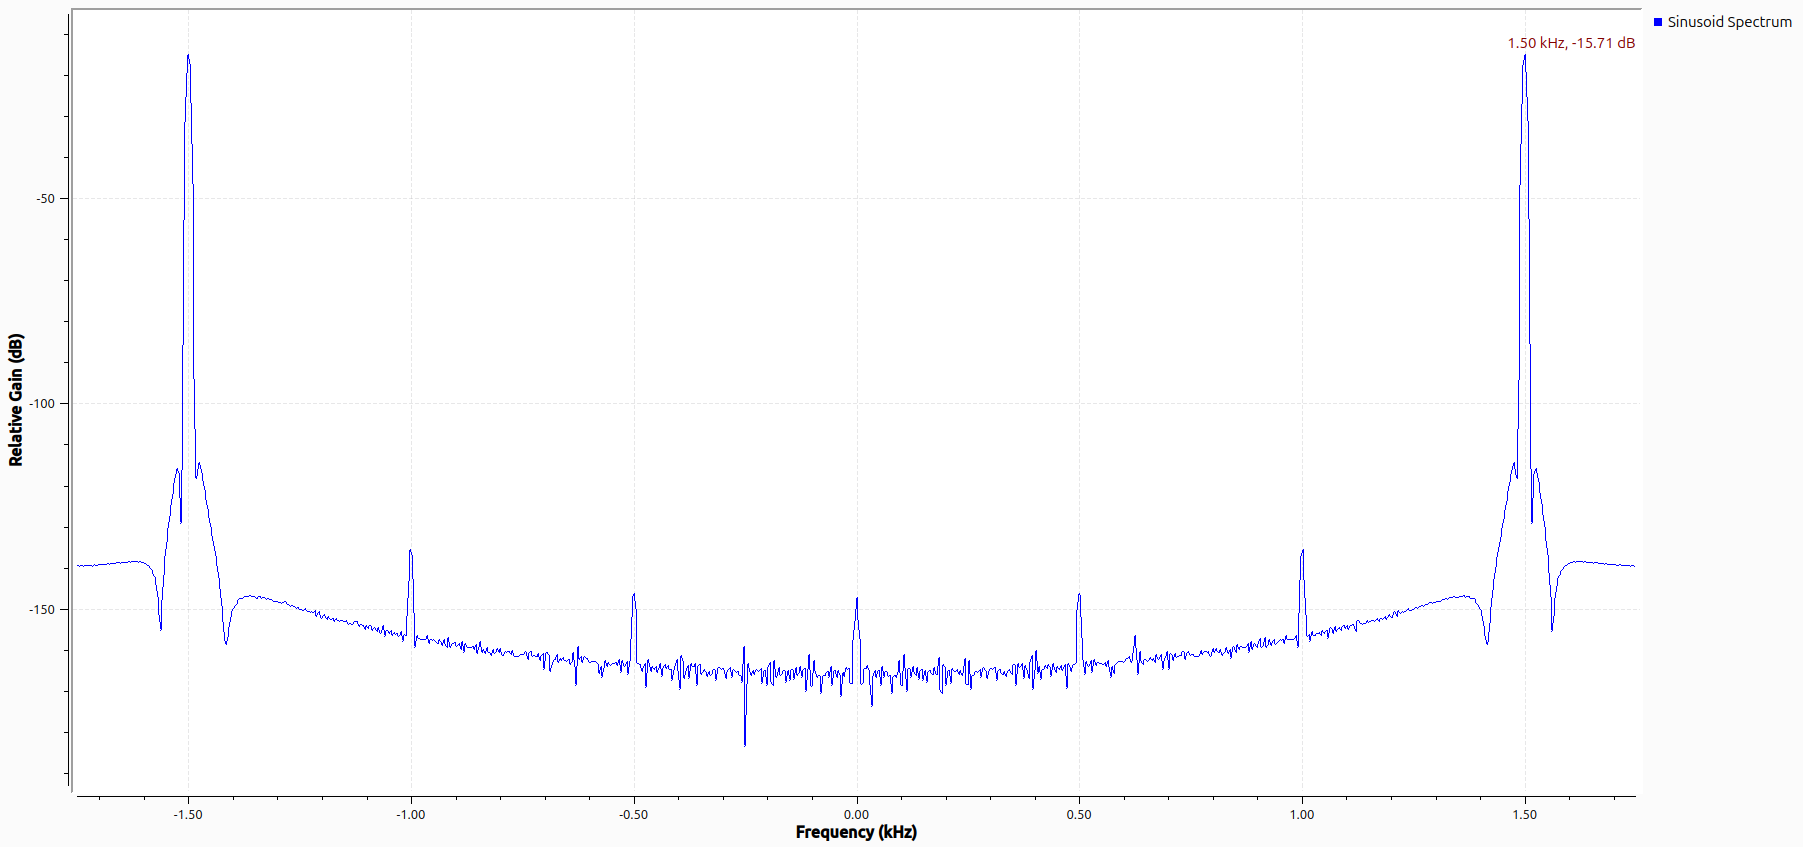
\includegraphics[width=0.7\textwidth]{sampling_rates_freq_domain_3_5k_samp_rate.png}}}
	\caption{Spectrum of Sinusoid Sampled at 3.5 kHz}
	\label{fig::sampling_rates_freq_domain_3_5k_samp_rate}
\end{figure}

The phenomenon we observe is called aliasing. The spectrum of a sampled signal wraps to $\pm f_s/2$. The delta function at positive frequency aliases from 2 kHz to -1.5 kHz and the delta function at negative frequency aliases from -2 kHz to 1.5 kHz. As a result, the measured frequency changes by 0.5 kHz, from 2 kHz to 1.5 kHz.

\subsection{Complex Sampling}

Using the flowchart shown in Figure \ref{fig::complex_sampling_experiment}, we investigate the effects of complex sampling. Figure \ref{fig::complex_sampling_freq_domain_10k_samp_rate} shows the updated spectrum.

\begin{figure}[H]
	\centerline{\fbox{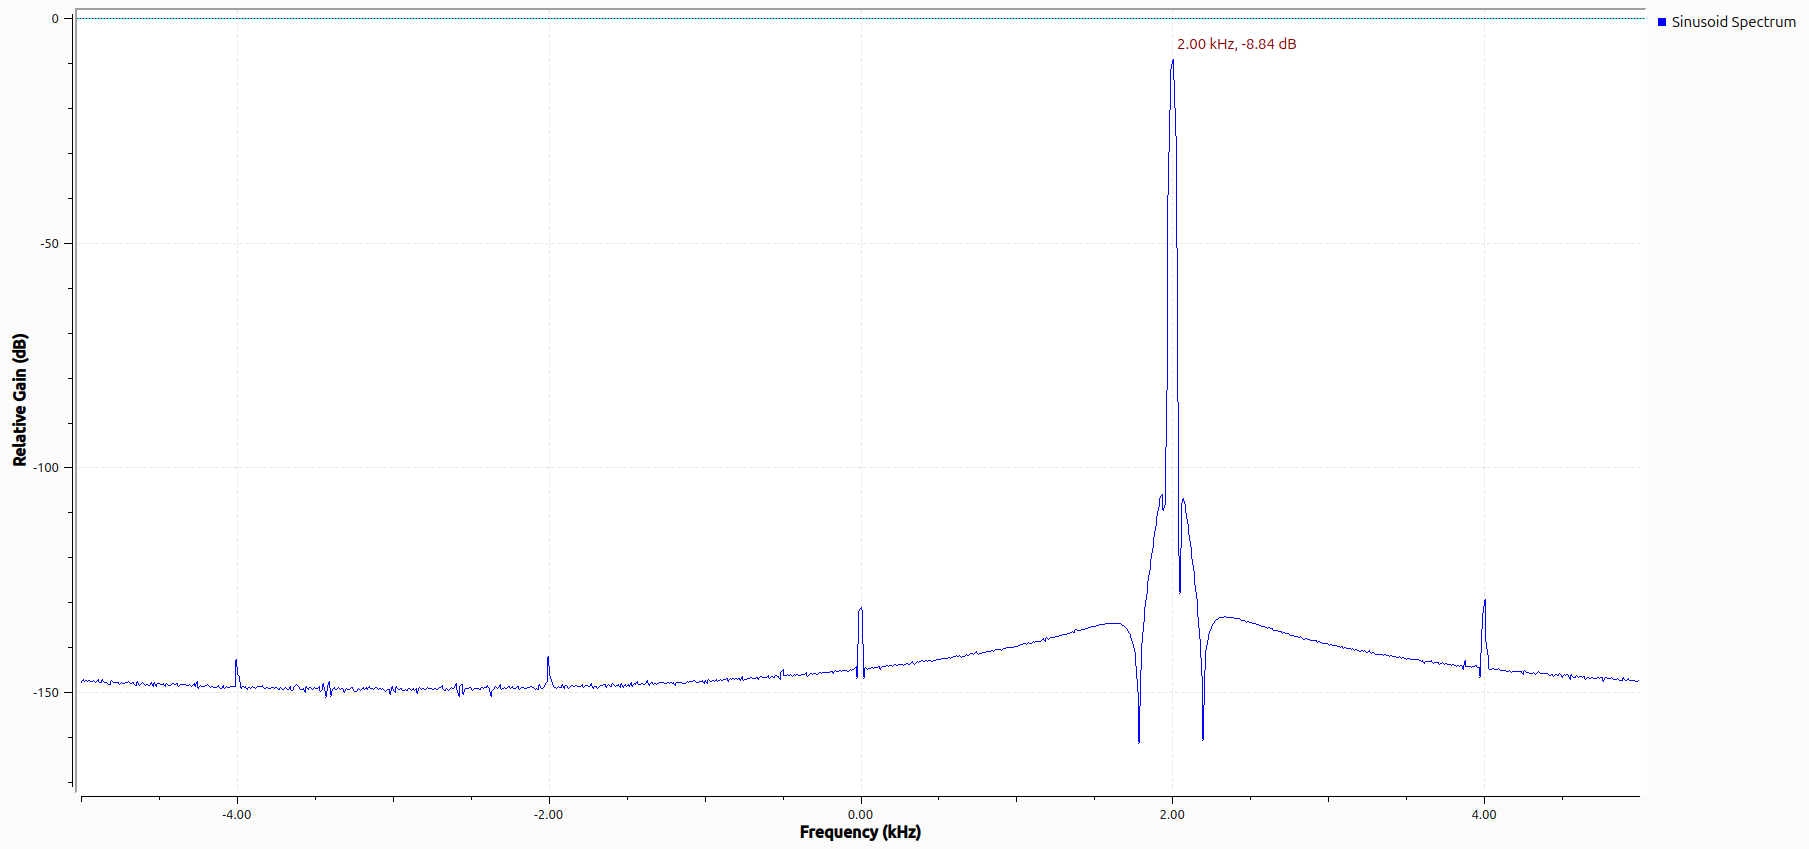
\includegraphics[width=0.7\textwidth]{complex_sampling_freq_domain_10k_samp_rate.png}}}
	\caption{Spectrum of Complex Exponential Sampled at 10 kHz}
	\label{fig::complex_sampling_freq_domain_10k_samp_rate}
\end{figure}

Compared to the spectrum shown in Figure \ref{fig::sampling_rates_freq_domain_10k_samp_rate}, the frequency response only has a positive component. This is expected because the frequency response of a complex exponential is a delta function. Compare this to a sine function, which can be expressed using the inverse Euler formula as:

\begin{equation}
	sin(2{\pi}{f_c}t) = \frac{e^{j2{\pi}{f_c}t} - e^{-j2{\pi}{f_c}t}}{2j}
\end{equation}

It is clear that a sinusoid can be decomposed into two complex exponentials with positive and negative frequencies resulting in a two-sided spectrum.

When viewed in the time domain, the captured data is composed of 2 channels as illustrated in Figure \ref{fig::complex_sampling_time_domain_10k_samp_rate}. These two channels represent the in-phase (I) and quadrature (Q) components of the signal. They serve as the real and imaginary parts of the complex data stream. The in-phase and quadrature components of the signal are 90 degrees out of phase.

\begin{figure}[H]
	\centerline{\fbox{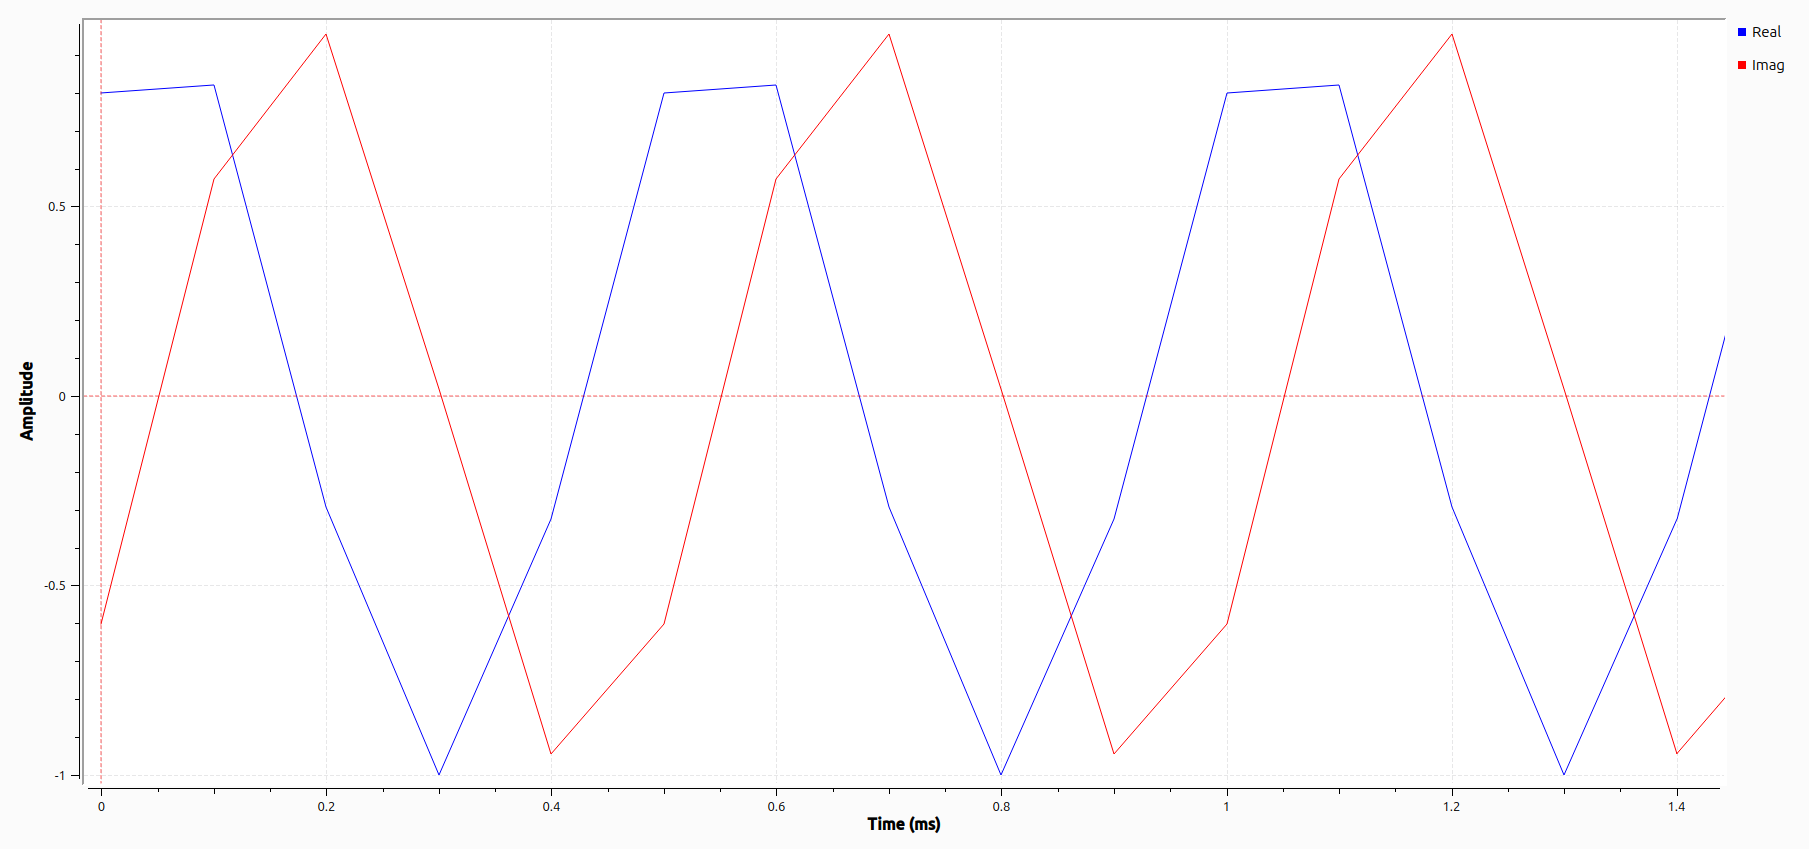
\includegraphics[width=0.7\textwidth]{complex_sampling_time_domain_10k_samp_rate.png}}}
	\caption{Time-Domain Capture of Complex Exponential Sampled at 10 kHz}
	\label{fig::complex_sampling_time_domain_10k_samp_rate}
\end{figure}

After increasing the sample rate to 40 kHz, we see that the amplitude of the real and imaginary parts of the signal are both 1 as expected. This result is captured in Figure \ref{fig::complex_sampling_time_domain_40k_samp_rate}.

\begin{figure}[H]
	\centerline{\fbox{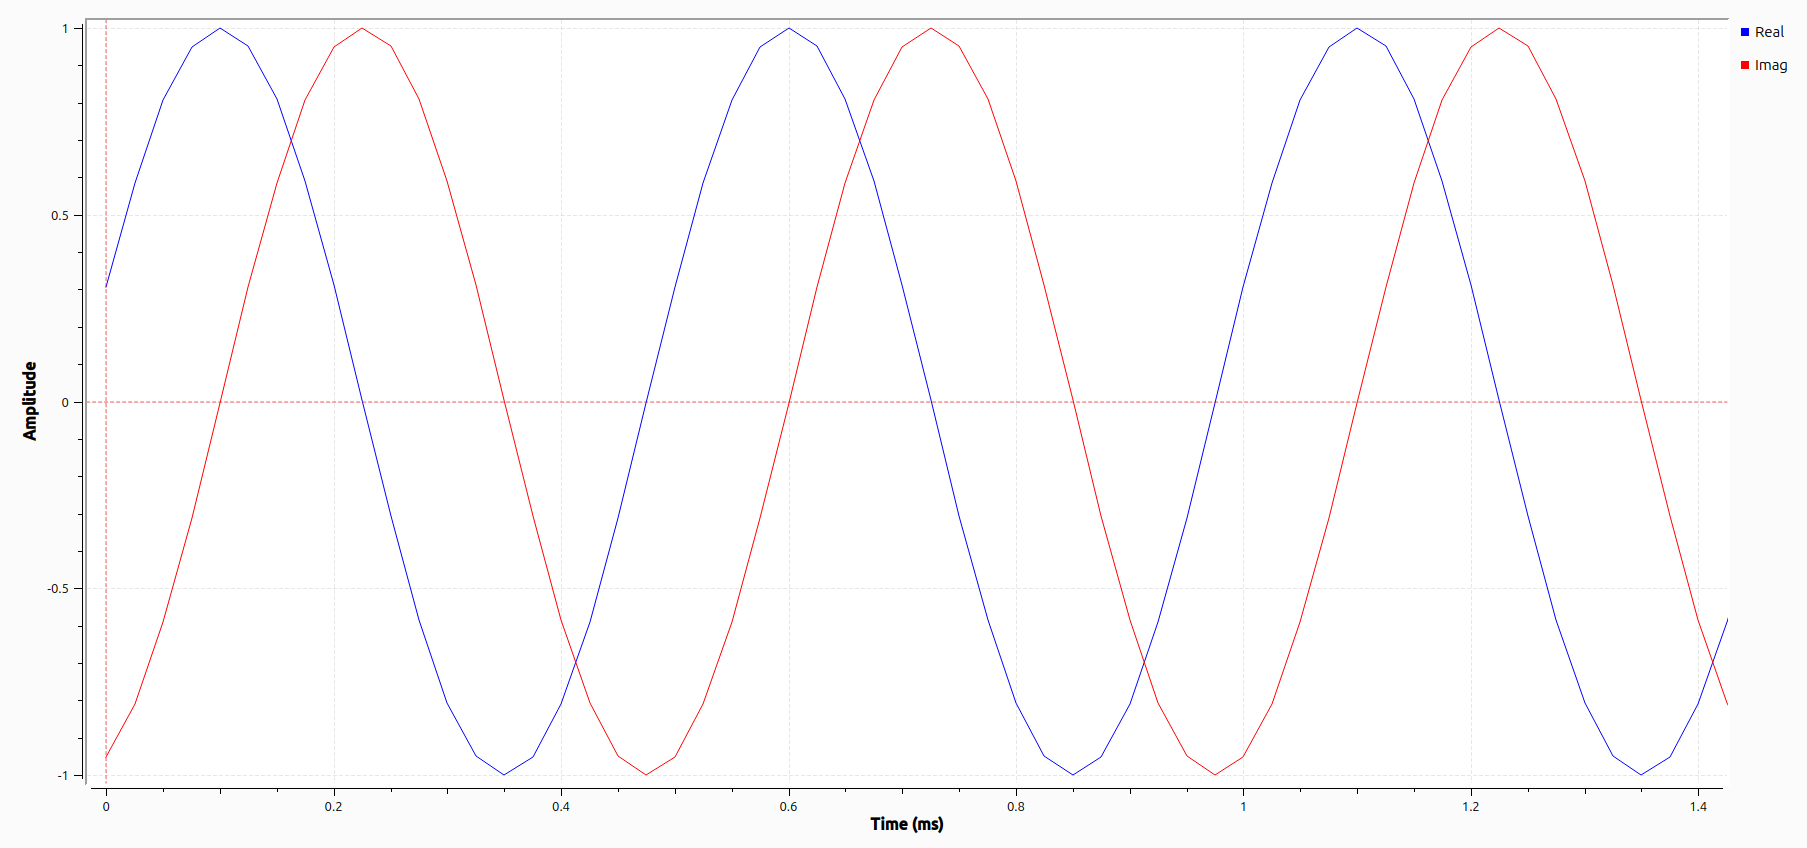
\includegraphics[width=0.7\textwidth]{complex_sampling_time_domain_40k_samp_rate.png}}}
	\caption{Time-Domain Capture of Complex Exponential Sampled at 40 kHz}
	\label{fig::complex_sampling_time_domain_40k_samp_rate}
\end{figure}

We can also measure the peak of the frequency response with the updated sampled rate as illustrated in Figure \ref{fig::complex_sampling_freq_domain_40k_samp_rate}. Doing so, we find a peak of 2 kHz, which is consistent with the data captured at a 10 kHz sampling rate.

\begin{figure}[H]
	\centerline{\fbox{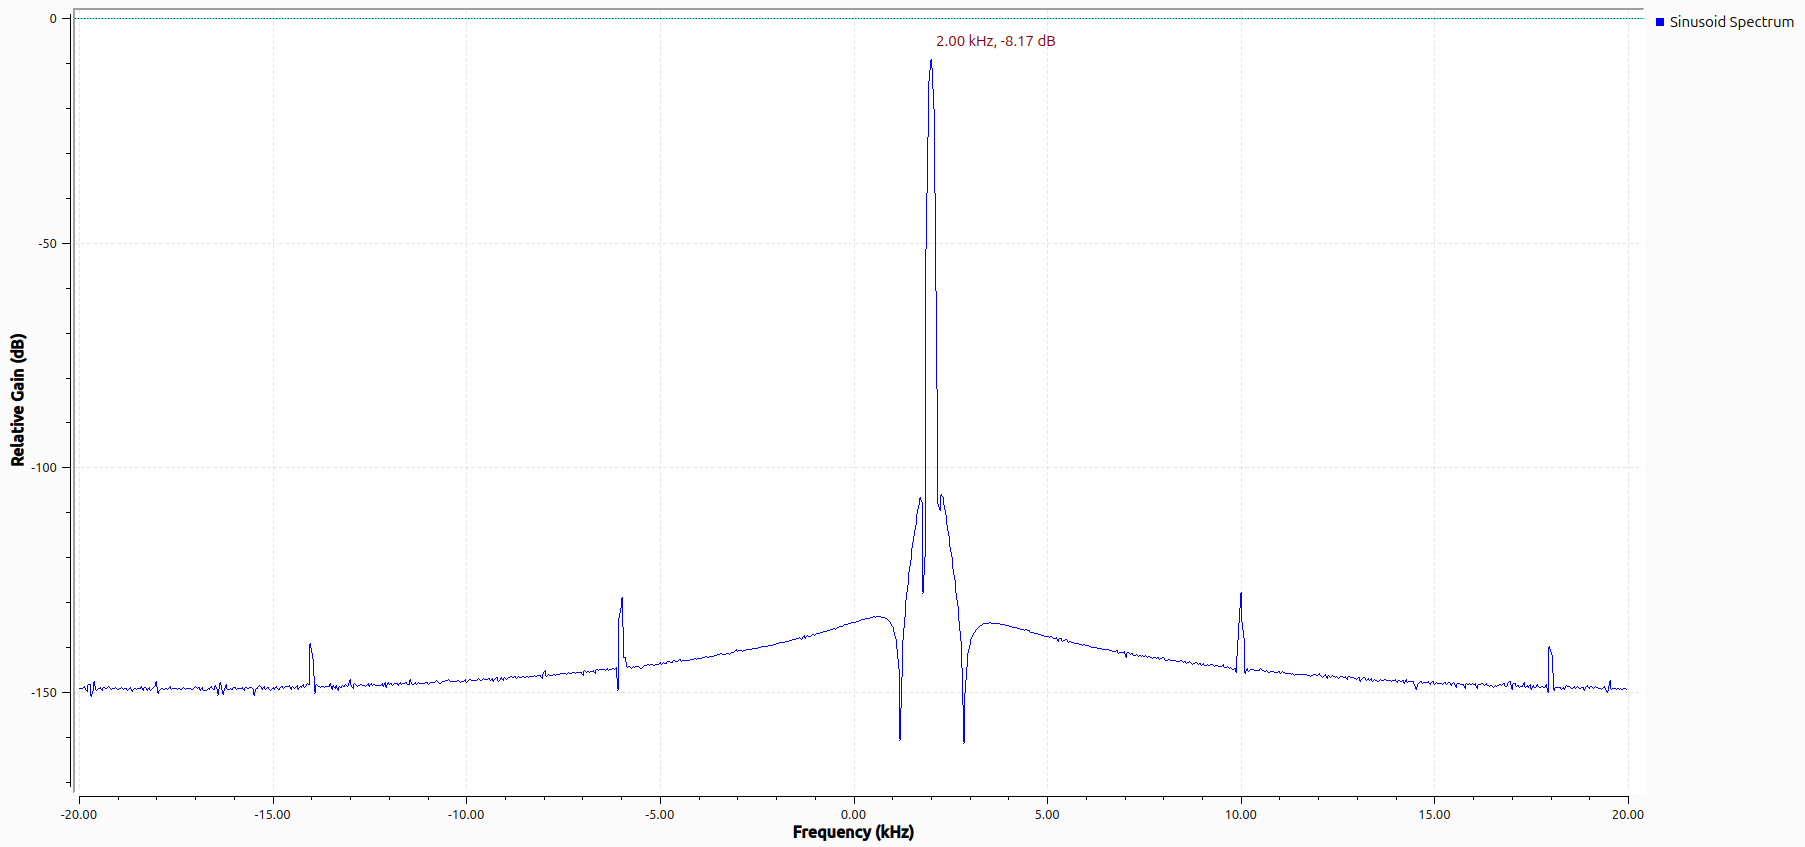
\includegraphics[width=0.7\textwidth]{complex_sampling_freq_domain_40k_samp_rate.png}}}
	\caption{Spectrum of Complex Exponential Sampled at 40 kHz}
	\label{fig::complex_sampling_freq_domain_40k_samp_rate}
\end{figure}

Next, we decrease the sampling frequency to the Nyquist rate of 4 kHz (twice the highest frequency) and recollect the frequency response. The updated frequency response is shown in \ref{fig::complex_sampling_freq_domain_4k_samp_rate} and peaks at $\pm 2 kHz$.

\begin{figure}[H]
	\centerline{\fbox{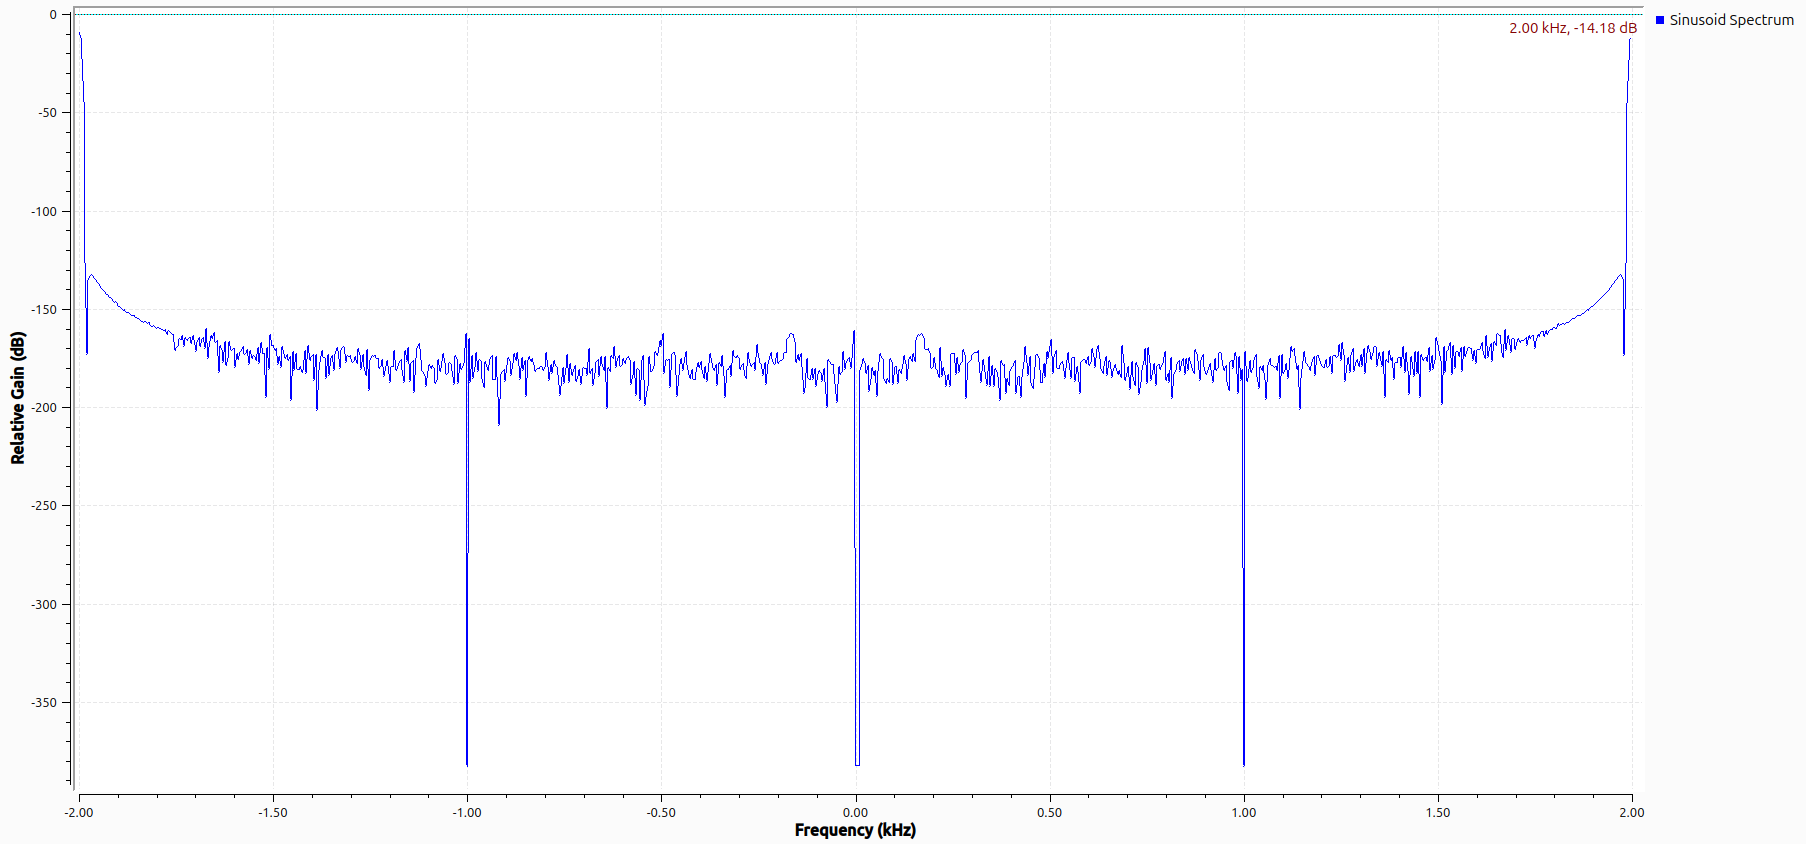
\includegraphics[width=0.7\textwidth]{complex_sampling_freq_domain_4k_samp_rate.png}}}
	\caption{Spectrum of Complex Exponential Sampled at 4 kHz}
	\label{fig::complex_sampling_freq_domain_4k_samp_rate}
\end{figure}

Our frequency response is captured using a windowed subset of samples. Since, we only use a subset of samples our delta function will morph into a function with a mainlobe, of measurable width, centered about the aliased carrier frequency. Due to the periodicity of the DTFT, what we are seeing is a copy of the mainlobe from different Nyquist zones. One is from the frequency response centered about 0 kHz and the other is from the frequency response centered at -4 kHz. We could also perform an inverse FFT shift on the data and interpret it using frequencies between 0 kHz and 4 kHz. This would make it easier for us to interpret the two frequency response peaks as a single peak.

\section{Conclusion}
Conclusions to the overall lab that discuss meaningful lessons learned and other takeaways from the assignment. (Important)

%sampling rates
%complex samples
%interpolation
%decimation
%noise analysis

%\title{Lab 1 - Introduction to Software-Defined Radio\\
%
\includegraphics[scale=0.25\textwidth]{ua_logo.png}}
%\author{Owen Sowatzke}
%\date{\today}
%\maketitle

\end{document}